%\cleardoublepage
\chapter{Introducción}
\label{sec:intro}
\pagenumbering{arabic} 

El aprendizaje automático (\emph{machine learning} o ML en inglés) es una rama de la Inteligencia Artificial y las Ciencias de la Computación que se centra en el uso de datos y algoritmos para imitar la forma en la que los humanos aprenden con el objetivo de aumentar gradualmente su precisión.
Es un componente fundamental del campo de la Ciencia de Datos, cuya importancia ha experimentado un gran crecimiento, especialmente en las últimas dos décadas \cite{cleveland2001}. 
El aprendizaje automático hace uso de métodos estadísticos y computacionales para entrenar algoritmos que realizan, entre otras tareas, clasificaciones o predicciones y que permiten descubrir piezas clave de información dentro de proyectos de procesamiento de datos. 
Posteriormente, esta información puede utilizarse en la toma de decisiones dentro de distintas aplicaciones y negocios, con una gran capacidad de impactar en el crecimiento de los mismos.

\section{Aprendizaje automático y consumo energético}

Gracias al desarrollo de nuevas tecnologías computacionales, el aprendizaje automático que se utiliza hoy en día es muy diferente de como era en el pasado.
El modelo actual surgió del reconocimiento de patrones y de la teoría de que los ordenadores pueden aprender a resolver tareas específicas, cuando los investigadores interesados en la Inteligencia Artificial se empezaron a plantear si los ordenadores serían capaces de aprender a partir de datos.
De aquí surge la importancia del aspecto iterativo de este aprendizaje, que permite que el sistema se adapte de forma independiente cada vez que nuevos datos son incorporados y sea capaz de aprender de cada computación previa para producir decisiones y resultados que sean confiables y repetibles.

Es así que, aunque una gran parte de los algoritmos utilizados en el aprendizaje automático son conocidos desde hace relativamente bastante tiempo, la habilidad de aplicar complejos cálculos matemáticos a grandes cantidades de datos una y otra vez, cada vez más rápidamente, es un desarrollo muy reciente conseguido gracias a los avances en componentes informáticos y la disminución de costes de grandes sistemas computacionales con enormes capacidades de memoria y procesamiento.
En especial, esto sucede en el campo del aprendizaje profundo (\emph{deep learning}), donde los modelos han crecido en cálculos para llegar a alcanzar típicamente el orden de los GigaFlops y en requisitos de memoria que se encuentran comúnmente en el orden de los millones de parámetros.

Sin embargo, este gran poder de procesamiento también trae consigo un gran gasto energético.
El consumo de energía en la arquitectura de computadores ha sido foco de atención de investigadores interesados en obtener procesadores energéticamente eficientes de última generación durante décadas. 
Por otro lado, los investigadores interesados en el aprendizaje automático se han centrado principalmente en la producción de modelos cada vez más profundos y precisos, sin poner ningún límite en términos computacionales más allá de la disponibilidad de procesadores capaces de llevar a cabo estos cálculos.

\begin{figure}[H]
  \centering
  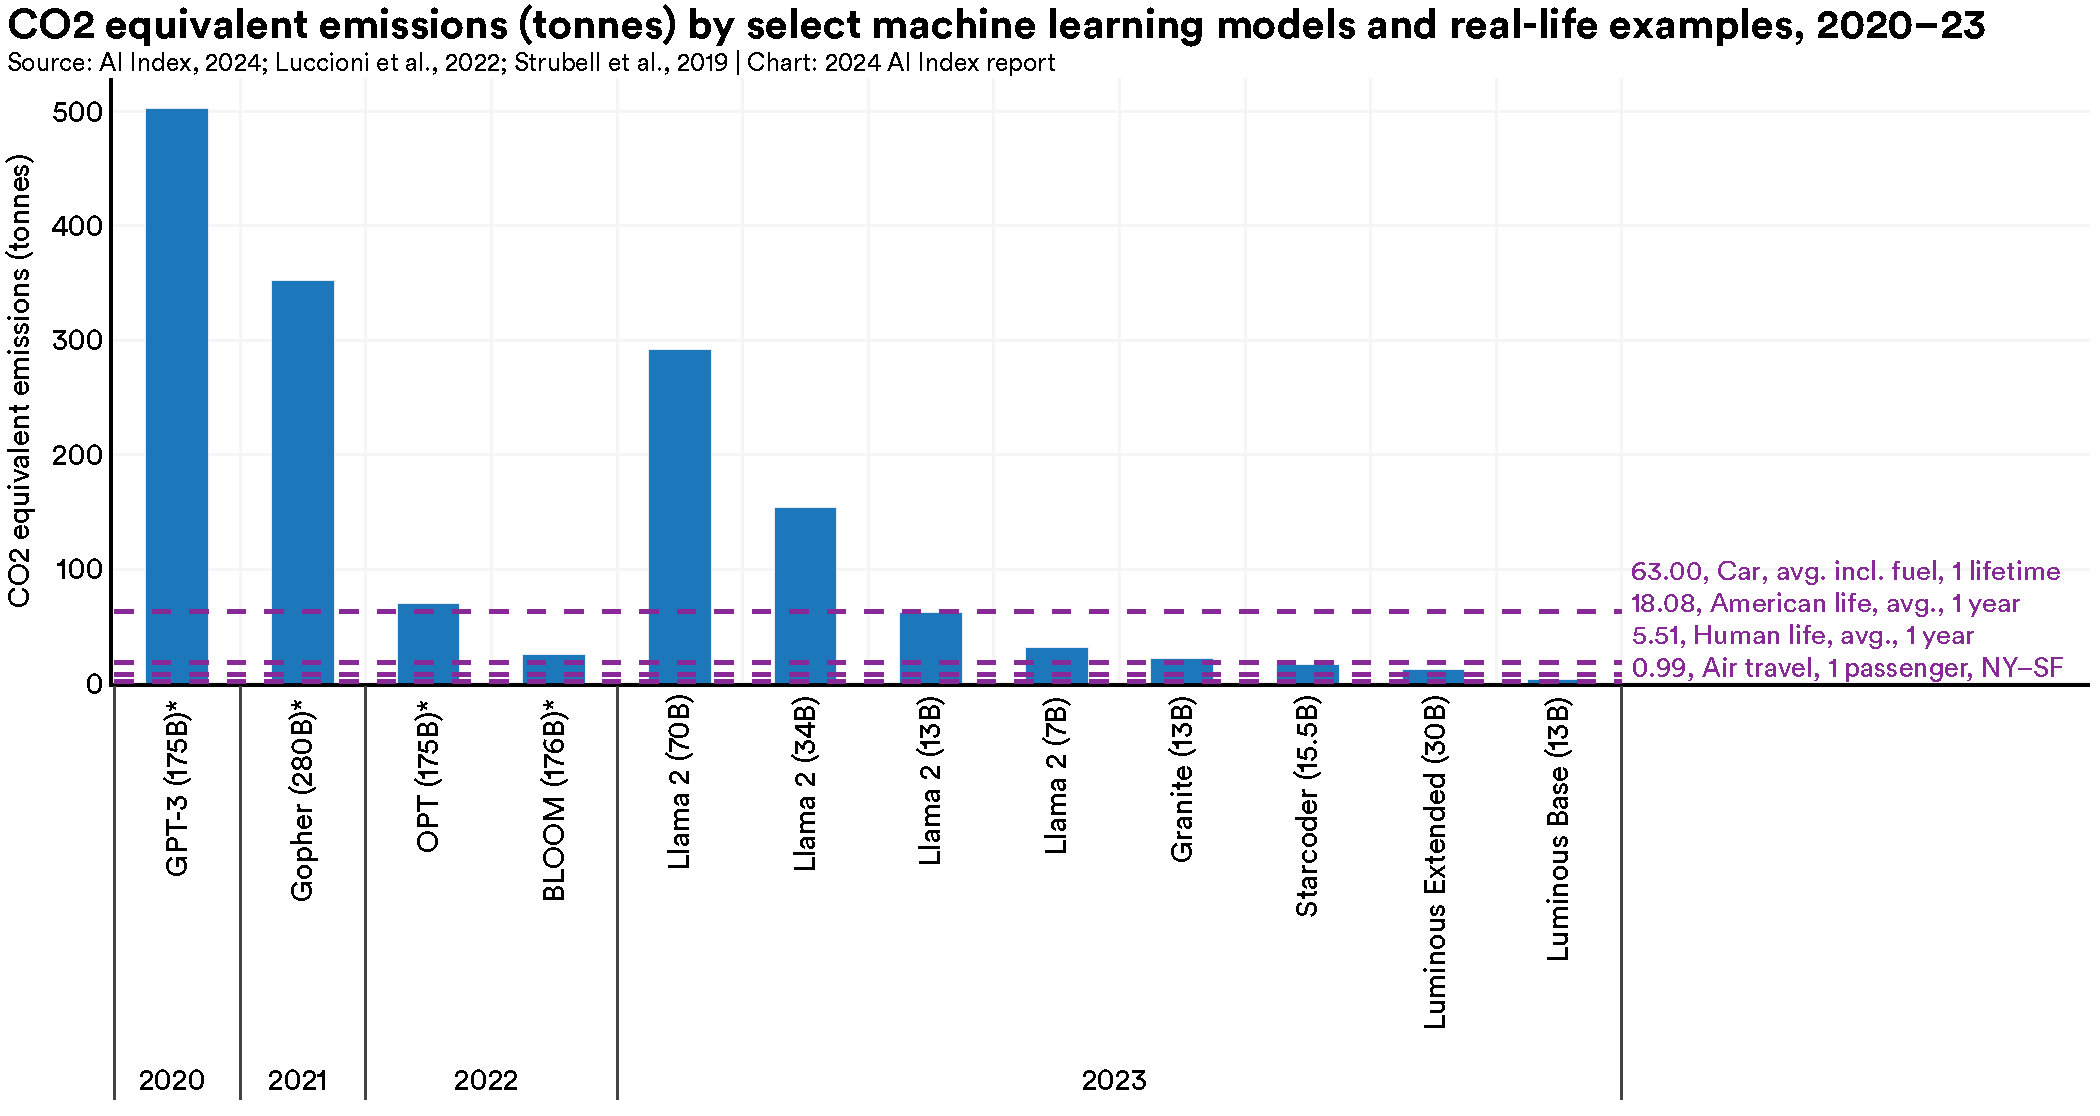
\includegraphics[width=\textwidth,keepaspectratio]{img/fig_2.13.1-ai-index.pdf}
  \caption{Emisiones de $CO_2$ producidas en el entrenamiento de varios modelos de gran escala en los últimos años. \\ Fuente: \citetitle{maslej2024aiindex} \cite{maslej2024aiindex}.}
  \label{fig:ai-index-emissions}
\end{figure}

Adicionalmente, con la reciente popularización de los grandes modelos de aprendizaje, especialmente de los modelos de lenguaje de gran escala (\textit{Large Language Models}, LLMs), pero también de la visión por computador y el aprendizaje en la nube, la investigación sobre el impacto energético se hace aún más necesaria. Los grandes modelos de lenguaje, por ejemplo, requieren enormes cantidades de datos y recursos computacionales para su entrenamiento, lo que se traduce en un consumo energético considerable \cite{samsi2023}. \mbox{GPT-3} \cite{brown2020language}, uno de los modelos más conocidos, cuenta con 175 mil millones de parámetros y requiere una cantidad masiva de energía para su entrenamiento. Del mismo modo, las aplicaciones de visión por computador, especialmente aquellas que involucran redes convolucionales profundas (CNN), también son intensivas en energía \cite{alyamkin2019low}. La figura~\ref{fig:ai-index-emissions} muestra las emisiones de $CO_2$ estimadas producidas durante el entrenamiento de varios modelos recientes, comparadas con referencias comunes como el consumo medio por una persona durante toda su vida.

El aprendizaje en la nube agrava estos problemas al trasladar el consumo energético a los centros de datos, que pueden tener diferentes niveles de eficiencia y fuentes de energía. Este tipo de aprendizaje, aunque ofrece flexibilidad y escalabilidad, puede tener implicaciones negativas para el consumo energético. Los centros de datos que alimentan estos servicios requieren grandes cantidades de electricidad, y su impacto depende en gran medida de la fuente de energía utilizada. Algunos centros de datos están migrando hacia fuentes de energía renovable para mitigar este impacto, pero la transición no es uniforme en todas las regiones.


\section{Desarrollo de una aplicación comparativa: \emph{MLCost}}

En este contexto temporal de modelos de aprendizaje que cada vez consumen más energía, se hace más necesario que nunca contar con una medida de la energía consumida y las emisiones producidas durante el proceso de entrenamiento. Esta información es vital para poder realizar una decisión informada en la elección de que modelos utilizar para una aplicación concreta de aprendizaje automático. Este proyecto propone el desarrollo de una aplicación, con el nombre MLCost, que permita a los investigadores obtener esta información de forma sencilla mediante el uso de herramientas existentes de medición. Para ello, la aplicación hace uso de librerías como CodeCarbon, que permite abstraer el método de calculo de emisiones, y Scikit-Learn, que permite entrenar modelos sin considerar gran parte del desarrollo de bajo nivel asociado con la implementación de los algoritmos utilizados y la preparación de conjuntos de datos para el entrenamiento. De este modo, la aplicación posibilita la medición del consumo y las emisiones producidas por distintos modelos a estudiar en cualquier conjunto de datos que se quiera utilizar, así como la comparación con gráficos sencillos de los resultados obtenidos.


\section{Objetivos del proyecto}
\label{sec:objetivos}

\subsection{Objetivo general}
\label{sec:objetivo-general}


Este Trabajo de Fin de Grado tiene como objetivo crear una herramienta que permita la comparación sistemática del consumo energético y el impacto de la huella de carbono en los modelos más representativos de técnicas de clasificación de aprendizaje automático supervisado.


\subsection{Objetivos específicos}
\label{sec:objetivos-especificos}

Para esta finalidad se han tenido en cuenta los siguientes objetivos específicos:

    \begin{itemize}
        \item Estudiar las herramientas disponibles para aprendizaje automático.
        \item Estudiar el uso de herramientas de medida del consumo energético.
        \item Comparar el consumo energético en los algoritmos de clasificación más importantes.
        \item Analizar la relación entre la precisión de los modelos y su consumo energético en conjuntos de datos de distintos tamaños y características.
    \end{itemize}

\section{Estructura de la memoria}
\label{sec:estructura}

La memoria de este proyecto se estructura en cinco capítulos, con una introducción, seguida de tres capítulos que reflejan las tres fases principales del proyecto: investigación, desarrollo y validación, para finalizar con las conclusiones y trabajos futuros.

El primer capítulo introduce el contexto en el cual se ha desarrollado la aplicación, proporcionando información de fondo y destacando los objetivos principales del proyecto. Este capítulo establece el escenario para los capítulos siguientes, ofreciendo una visión general del alcance y propósito del proyecto.

El segundo capítulo revisa la literatura relevante y el estado del arte en cuanto a métodos de medición de emisiones y estudios sobre el consumo energético del aprendizaje automático. Además, proporciona una introducción general al aprendizaje automático, describe las librerías existentes utilizadas en el desarrollo del proyecto y detalla los modelos y conjuntos de datos utilizados durante las pruebas de la aplicación.

El tercer capítulo describe la arquitectura de la aplicación desarrollada, incluyendo el proceso de preparación de los datos y los métodos de evaluación de las predicciones de los modelos. Este capítulo se centra en los aspectos técnicos del diseño y la implementación, explicando las decisiones de diseño y cómo se implementaron las diferentes funcionalidades.

El cuarto capítulo recoge todas las pruebas realizadas con la aplicación, incluyendo dos experimentos concretos. El primero compara varios modelos en distintos conjuntos de datos de creciente complejidad, mientras que el segundo compara varios modelos en diferentes máquinas con diversos recursos de procesamiento. Este capítulo detalla la metodología de los experimentos y presenta los resultados obtenidos, analizando el impacto del consumo energético en el rendimiento de los modelos.

El último capítulo concluye la memoria resumiendo los principales hallazgos del proyecto y evaluando el grado de consecución de los objetivos planteados. Además, este capítulo incluye una reflexión sobre el conocimiento adquirido y sugiere posibles direcciones para trabajos futuros, proponiendo mejoras y ampliaciones a los estudios realizados.

%\cleardoublepage